% capitulo1.tex
\chapter{Introducción}

La manera en que se entregan contenidos audiovisuales a los auditores en la actualidad son el resultado de más de un siglo de evolución en materia tecnológica, tanto para el registro de la información, imagen y/o audio, como para las vías de comunicación. Esta evolución está compuesta de hitos científicos que datan del siglo XIX, y entregan una historia rica en avances e investigación destinada al desarrollo de sistemas que entregan información de la mejor forma posible.\\

A lo largo de los años estos desarrollos han significado un cambio en el comportamiento de los auditores, que a su vez han generado o destruido industrias relacionadas a los contenidos audiovisuales. Considerando que el fin de este proyecto de memoria busca implementar una nueva forma de entregar contenido utilizando parte de la tecnología actual, es necesario revisar los sucesos desde el génesis de los registros y comunicación de medios audiovisuales.


%La relación entre el registro de datos audiovisuales y las comunicaciones se han relacionado desde inicios del siglo XIX, es decir 

%El fin de este proyecto es lograr la entrega de contenidos audiovisuales a una nueva audiencia que ha surgido con los últimos avances tecnológicos del siglo XXI, específicamente Internet y la telefonía móvil. 
%La entrega de información a gran escala se encuentra constantemente asociada a los avances tecnólogicos para el registro de imagenes y audio.
%A través de los años el registro de datos de imagen y audio, se ha asociado a la entrega del contenido a una gran cantidad de personas, o auditores. Por lo tanto se deba abordar el inicio de estos registros a el estado actual de las transmisiones.

%Previo al desarrollo del proyecto se debe tener presente la historia y avances tecnológicos relacionados con las transmisiones de medios.

%La historia de los medios es importante por cuanto comprende los avances logrados por el hombre que nos permitieron arribar a los resultados tecnológicos actuales. Lo anterior toda vez que así como la historia de todas las instituciones sociales políticas y económicas del hombre han evolucionado a través de la historia, es la tecnología donde las escalas de avance se han dado en forma más notoria sobre todo en el pasado siglo XX, desde donde por ejemplo de la comunicación por carta manuscrita se logró la comunicación cablegráfica, a mayor abundamiento en materia eléctrica, se logró en menos de 70 años de elevar en vuelo a 2 hombre 1,5 km a poner al hombre en la luna.
\section{Historia de los medios}
%Introducción nueva
%¿Qué son las redes de sensores inalámbricos?
Tomando en cuenta que desde sus inicios la reproducción de medios siempre ha estado relacionada con los últimos avances científicos, los medios de distribución actuales tienen sus orígenes en avances que datan  del siglo XIX.\\

Inicialmente los registros de audio con posibilidades de distribución aparecieron con el invento basado en el fonógrafo de Thomas Alva Edison, como también en el Gramófono de Emile Berliner, aparecido en 1887 y patentado en 1888. La diferencia con el diseño original de Edison está en el medio de registro de audio con el disco de vinilo. Cabe recordar la famosa imagen de la compañía RCA Víctor del Perro escuchando la voz del amo.\\

Análogamente el registro de imágenes en movimiento apareció gracias al cinematógrafo, invento del francés Léon Bouly, y más tarde desarrollado y popularizado por los hermanos Auguste y Louis Lumière, el cual permitió la grabación y reproducción del contenido con la misma máquina.\\

Esta tecnología sienta bases para la transmisión de contenidos a gran escala, \textit{broadcasting}. Para el siglo XX, los avances en tecnología permiten experimentar con difusión a través del espectro de frecuencias.\\

 Ya en el año 1920 la radio es el medio más popular de difusión, llegando a estar presente en 40 millones de hogares estadounidenses, para tres décadas después, en los 1950’s ser reemplazada en popularidad por la transmisión de imágenes y sonidos a través de la naciente televisión.\\

	Estos medios comunicativos para la década actual mantienen su esencia, que es la transmisión del video y/o audio a un gran universo de personas. Si bien el medio por el que se transmite, la resolución, fidelidad, formato y tamaño de los equipos han cambiado, las bases que las fundamentan siguen siendo la transmisión de contenido audiovisual a una gran cantidad de personas, ya sea con fines informativos, de educación o entretención.\\
	
En la actualidad las transmisiones de audio y video se encuentran en un estado de transición desde medios de comunicación análogo como, por ejemplo, la radio FM, AM y la televisión PAL, NTSC, SECAM, a transmisiones digitales. El motivo de este cambio tecnológico es aprovechar de mejor manera el espectro radioeléctrico, enviando la misma o mayor información que por transmisiones análogas, pero utilizando menos recursos del espectro (Subtel Chile \cite{sota:subtel}).\\

Otro medio de transmisión y comunicación global que ha tomado gran significancia en la última década es la Internet. A través de transmisiones de flujos de datos (\textit{streaming}), es posible escuchar radios online, ver videos en YouTube, o utilizar servicios de películas “on-demand” como Netflix, por dar ejemplos disponibles en Chile. Todo esto siendo recibido en un computador u otro dispositivo que presente conectividad a la red.\\

Estos dispositivos alternativos tienen el peso de llevar la recepción de medios audiovisuales por un nuevo rumbo y ya están siendo considerados por las empresas que generan el contenido, al proveer salidas directas a televisores con Internet; consolas de videojuegos con navegador web o aplicaciones cliente para servicios de audio o video on-demand. Otro punto a tener en cuenta es la mayor importancia que tiene el crecimiento del consumo de dispositivos móviles como celulares o reproductores portátiles multimedia, donde se puede llegar a una audiencia aun mayor.\\

Considerando el gran papel que está tomando Internet en el consumo de contenidos, es necesario enfocar el desarrollo de las transmisiones a resultados que aprovechen este medio y llegar así a la creciente audiencia que lo utiliza. 
Esto aportaría en el futuro a igualar o incluso superar en importancia a las transmisiones por internet con las del medio terrestre, tanto digitales como análogas.

\clearpage
\section{Tecnología actual relacionada}
En la siguiente sección se presentan las tecnologías actualmente en uso para la transmisión de medios.

\subsection{Estado actual de las transmisiones}

Considerando que el objetivo de este trabajo tiene relación con la distribución y recepción de contenidos audiovisuales se presentan distintos medios funcionando actualmente.\\

\subsubsection{Video-on-demand}
Es un servicio de distribución que permite a los usuarios seleccionar y ver o escuchar contenidos de video o audio de manera personalizada, ofreciendo la opción de solicitar el material en el momento exacto que lo desee.  La plataforma para poder reproducir el contenido se puede encontrar implementada como aplicación en un computador o a través de un dispositivo con conexión directa al televisor y al proveedor del servicio. En Chile este servicio es provisto por la compañía VTR a través de su dispositivo D-Box, este dispositivo cumple además la función de DVR.\\

La compañía Netflix también provee este servicio, sin embargo el medio de transmisión es Internet, ofreciendo a sus clientes suscripciones que permiten el acceso al catálogo de películas y documentales.\\

En Chile el servicio de \textit{Video-on-demand} entregado por Netflix se ha posicionado a partir de Septiembre de 2011 buscando simplificar el registro de nuevos usuarios, su potencial captación de nuevos usuarios se magnifica al poner a disposición de sus clientes el acceso a los contenidos a través de variadas plataformas de reproducción, como consolas de videojuegos de sobremesa: Nintendo Wii y PlayStation 3, consolas portátiles como Nintendo 3DS, acceso vía web y aplicaciones para televisores con InternetTV. \\

\subsubsection{Podcast}
Es una serie de archivos de medios digitales (audio o video) lanzados en forma periódica por episodios, este sistema permite al usuario descargar el material de su interés para poder reproducirlo más tarde.\\

El modo de distribución se diferencia de otras formas de transferencia de internet como lo son la descarga directa al estar todos los archivos catalogados en un servidor central, éste además provee a los usuarios una vía de distribución a través de RSS Feeds, que son archivos de información en XML (\textit{extended markup language}) diseñados para compartir actualizaciones de sitios web, popularizados por los blogs.\\ 
El uso de RSS Feed para los podcast permite informar a los suscriptores de nuevos contenidos, aunque no es necesario que la persona esté suscrita para obtener alguna información en especifico. 
Su uso se ha popularizado por la plataforma iTunes desarrollada por Apple, que en su versión 4.9 de 2005, abrió a una gran base de usuarios este nuevo medio de comunicación. No solo se utiliza para entregar programas de radio, sino que también documentos y programas de televisión, de manera gratuita.\\

\subsubsection{Streaming media}
Este método provee constantemente datos multimedia al usuario final, que puede reproducir mientras el servidor se encuentra entregando la información.
El nombre se refiere a que el método de entrega es continuo, sin interrupción, debido a que los datos recibidos se almacenan en un buffer de memoria que se va liberando mientas se reproduce. Es decir los datos de audio o video, no son descargados,  es un acceso directo al contenido intangible.\\

Un uso más reciente que se le ha dado al método streaming es lo que se llama \textbf{\textit{LiveStreaming}}, donde el contenido a distribuir es capturado en el momento, una transmisión en vivo que es posible de ser recibida por el usuario casi al momento que ocurre gracias al flujo o stream de datos.\\

La base fundamental de este método de distribución, es la utilización de protocolos ligeros de la capa de transporte, como lo es UDP (\textit{User Datagram Protocol}) que a diferencia del protocolo TCP (\textit{Transmission Control Protocol}), no asegura la entrega en caso de fallo, permitiendo obviar los paquetes, priorizando la continuidad del flujo en el tiempo sobre la fiabilidad de los contenidos.  En la capa de aplicación se ha desarrollado un protocolo con este objetivo, toma como base la conexión mediante UDP para realizar el enlace, es llamado RTP (\textit{Real-time Transport Protocol} \cite{sota:rtp-draft}).\\

Sin embargo existe un protocolo de capa de aplicación desarrollado para realizar transmisiones de \textit{LiveStreaming} a través de un enlace por TCP llamado \textit{Real Time Messaging Protocol} (RTMP \cite{bib:rtmp-specs}), éste fue hecho por la empresa Macromedia, siendo ahora propietario \textbf{Adobe Systems}. Se destaca por lograr streaming multimedia con baja latencia gracias al envío de una gran cantidad de fragmentos del stream con una pequeña cabecera. \\

%Aun así existe un protocolo de la capa de aplicación que utiliza TCP para realizar el enlace. Este fue desarrollado originalmente por Macromedia, siendo ahora propietario \textbf{Adobe Systems}. \textit{Real Time Messaging Protocol} (RTMP \cite{bib:rtmp-specs}) fue desarrollado para realizar streaming multimedia a través de TCP con baja latencia, esto lo logra gracias al envío de la mayor cantidad de información por enlace. \\
	
	De forma similar al protocolo RTMP \textbf{Apple Inc.} ha desarrollado un nuevo método llamado \textit{\textbf{HTTP Live Streaming}}, se diferencia al utilizar pedazos de audio o video  ordenados en una lista de reproducción de extensión \textbf{m3u} (\cite{sota:m3u-specs}) manteniéndose actualizada a medida que nuevos contenidos son creados. A diferencia del \textit{streaming} nombrado anteriormente, este flujo de datos se transmite a través del protocolo HTTP (\textit{Hypertext Transfer Protocol} \cite{sota:rfc-http}), el cual siendo de una capa superior (de aplicación) posibilita la transferencia de los datos multimedia con un servidor web ordinario, como por ejemplo Apache. Además permite la transmisión en redes donde firewalls o proxies puedan bloquear el contenido, ya que se enmascara como tráfico de hipertexto. Cabe destacar que el enlace realizado a través del protocolo de la capa de aplicación HTTP utiliza TCP en su capa de transporte, al igual que RTMP.


\subsection{Almacenamiento del Contenido}

Otra tecnología relacionada son los llamados \textbf{DVR} (\textbf{digital video recorders}), dispositivos interactivos que cumplen con la grabación de la señal de televisión o video, siendo almacenada en formato digital.\\

 Esta información queda guardada en el disco duro o memoria del sistema, para poder ser vista después. A diferencia de una antigua videograbadora, el medio de almacenamiento y el formato es digital, permitiendo tomar registro y así manipularlo mediante software.\\
 
	El concepto es aplicado en hardware para televisión e implementado en decodificadores de televisión pagada. En el caso de proveedores de cable, la transmisión es recibida por el enlace coaxial, donde el dispositivo cumple la función de decodificar la señal digital y almacenarla si posee características de DVR.

\subsection{Registros de Stream}

Se puede implementar este concepto de DVR en software de computadores de escritorio, desarrollando alguna aplicación que permita registrar los segmentos transmitidos por streaming para ser reproducidos en otra ocasión. \\

	Servicios de streaming populares como Justin.TV, UStream o Twittcam permiten transmitir video a través de sus plataformas web, y permiten la revisión del contenido tiempo después que éste ha finalizado. En cierta parte este comportamiento se asemeja al DVR, pero no posibilita moverse en el tiempo mientras se transmite.\\

En Chile, se ha desarrollado una aplicación más sofisticada por parte de la empresa AltaVoz S.A. con su proyecto \textquotedblleft SocialStream, Video TimeShift\textquotedblright \ , el cual permite retroceder y revisar el contenido mientras la transmisión se encuentra en curso. Este registro es encargado al servidor quien administra los pedazos de información multimedia, una aplicación cliente entabla conexión para realizar pedidos de la información en el tiempo que desea el usuario.
Esta característica lleva como nombre \textbf{\textit{TimeShift}} \cite{cap1:time-shift}, sin embargo la empresa utiliza el nombre \textbf{Janus} \cite{cap1:altavoz-janus} para comercializarla.

\section{Propuesta de Proyecto}
\subsection{El Smartphone}
Un \textit{Smartphone} es un teléfono portátil con conectividad a las redes celulares y que presenta características adicionales respecto a los teléfonos móviles comunes.\\

Sus bases se sientan en los siguientes conceptos:
\begin{itemize}
\item Su funcionalidad puede ser extendida a través de aplicaciones adicionales.
\item Debe poseer un teclado QWERTY físico o virtual.
\item Debe permitir estar siempre conectado a la Internet.
\end{itemize}
Considerando estos conceptos se puede encasillar como Smartphone a los teléfonos Blackberry, iPhone y Android.

\subsection{Trasfondo}
La mayoría de los smartphones permiten el acceso a Internet a través de la red celular utilizando distintas tecnologías de transmisión de datos (no sólo WiFi), como lo son actualmente EDGE, HSPA y LTE \cite{cap1:tecnologias-celulares}. Estas se encuentran en incesante desarrollo, presentando mejoras en la velocidad de transferencia de datos.\\

La constante mejoría en la velocidad de transmisión en redes celulares ha permitido la reproducción de contenidos multimedia. Un avance similar a lo experimentado en la década de 1990 por los computadores multimedia de escritorio. En primera instancia con aplicaciones de contenido audiovisual (imagen, audio, video, texto) ejecutadas localmente, para luego evolucionar y llegar a recibir y transmitir este contenido a través de la \textit{World Wide Web}.\\

Los smartphones actuales ejecutan sistemas operativos avanzados que proveen módulos de conexión  a redes, ya sea celular, WiFi, o Bluetooth, si es que el hardware lo incorpora. Además de navegadores web diseñados especialmente para estos dispositivos, con características como presentar en pantalla reducida o ajustada a la resolución, interfaz táctil, teclado numérico, etc.\\

Considerando estas dos importantes bases, conectividad y sistema operativo capaz, es posible implementar una aplicación que se asemeje a la experiencia en computadores de escritorio.\\

\subsection{La Problemática}
El producto desarrollado por la empresa chilena AltaVoz S.A.: \textbf{SocialStream}, destinado a computadores de escritorio y aparatos de sobremesa consiste en una herramienta que permite registrar en el momento, una transmisión en vivo de audio o video. Posibilita al consumidor del contenido, retroceder a un punto en específico, pausar  y avanzar (limitado por el punto más reciente de la transmisión). 
A diferencia de dispositivos de sobremesa (\textbf{set top boxes}) como lo son TiVo u otros DVR, el registro de la transmisión es encargado al servidor quien provee los contenidos a los clientes que se han conectado, y estos contenidos no son guardados localmente. \\

Este sistema nos significan los siguientes beneficios: 
\begin{itemize}
\item Ahorro para el consumidor, espacio en sus dispositivos de almacenamiento
\item Cierto control del proveedor sobre la distribución  y copia de los contenidos
\item La posibilidad de portar a otras plataformas como consolas de videojuegos o dispositivos móviles.
\end{itemize}

Las bases de esta herramienta se fundan sobre Adobe Flash gracias a su protocolo RTMP, y considerando las diferencias tecnológicas entre Apple y Adobe (ver \cite{sota:steve-flash} carta de Steve Jobs, ex-CEO de Apple Inc.) surge el problema principal:

\begin{itemize}
\item Las aplicaciones que cumplen la función de reproducción para este producto están desarrolladas en el lenguaje de programación ActionScript, propio de Adobe.
\item En las plataformas de escritorio y algunos smartphones, esto no significa un problema. Sin embargo los dispositivos de Apple con el sistema operativo iOS no presentan compatibilidad con estas tecnologías Flash.
\end{itemize}

	En las siguientes figuras se puede notar claramente el problema que genera en iOS la falta de soporte de tecnologías Adobe. 
	En la captura de pantalla del navegador web de un celular con el sistema operativo Android (\ref{sshot_Android_sstream}) se presenta de forma íntegra la página web, nótese que el reproductor hecho con tecnología Flash se presenta de la misma forma que en un navegador web de computador de escritorio. 
	En la siguiente captura Mobile Safari (\ref{sshot_iOS_sstream}) presenta el problema de la falta de soporte para Flash, la página web muestra sus componentes HTML ausentando el reproductor de video.

%\clearpage 
\begin{figure}[h!]
	\centering
	% \fbox{ } % la encierra en un cuadrado, sirve para código también
	 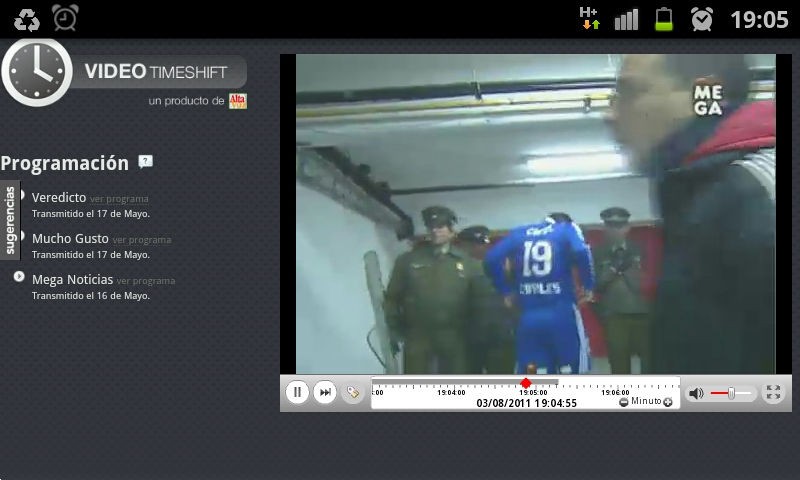
\includegraphics[scale=0.47]{imgs/sshot_Android_sstream.jpg}
 	\caption{Reproducción de SocialStream en Android OS.}
	\label{sshot_Android_sstream}
\end{figure}
%\vspace{3cm}
\begin{figure}[h!]
	\centering
	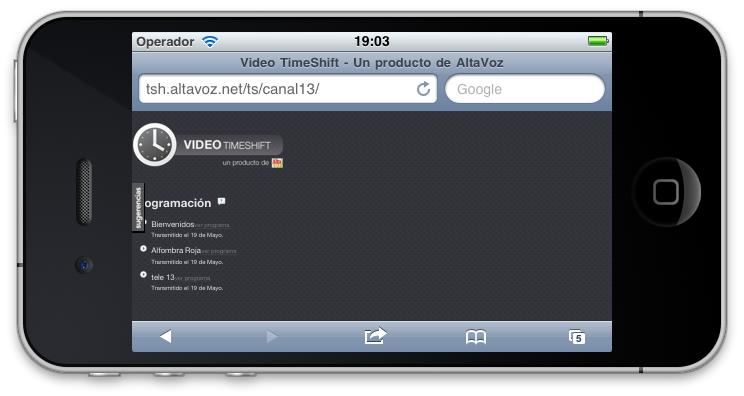
\includegraphics[scale=0.55]{imgs/sshot_iOS_sstream.png}
	\caption{Reproducción de SocialStream en iPhone con iOS}
	\label{sshot_iOS_sstream}
\end{figure}

\newpage
\subsection{Posibles Soluciones}

Las herramientas de distribución de audio y/o video por streaming están limitadas a los reproductores provistos por la interfaz de programación de aplicaciones (API) de iOS. El reproductor por defecto del sistema operativo permite reproducir un stream multimedia dando la posibilidad de retroceder la reproducción según el contenido disponible en el buffer de datos del mismo reproductor, este tiempo se limita a 30 segundos.

%\clearpage
\begin{figure}[h!]
	\centering
	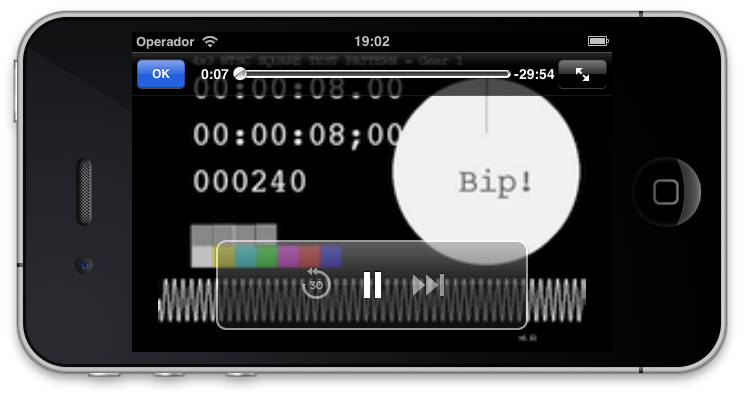
\includegraphics[scale=0.55]{imgs/sshot_iOS_hls.png}
	\caption{Reproducción de flujo video por HTTP Live Streaming}
	\label{sshot_iOS_hls}	
\end{figure}

De la figura \ref{sshot_iOS_hls} se puede notar el botón a la izquierda en la barra inferior de  la pantalla, este hace retroceder en 30 segundos la reproducción.\\

Esta característica es propia del componente \textit{MPMoviePlayerController} del marco de trabajo de la API de iOS \textit{\textbf{MediaPlayer Framework}} \cite{cap1:mediaplayerframework}, éste simplifica de gran manera la necesidad de mostrar video o reproducir audio en el dispositivo.\\

Se debe dejar claro que Apple es sumamente restrictivo en el uso de la API de iOS debido a que velan que sus componentes sean utilizados por los programadores de la forma que ellos establecieron originalmente. Para controlar el comportamiento de las aplicaciones publicadas en la tienda de aplicaciones App Store los desarrolladores deben pasar por un proceso de revisión basado en las \textbf{directrices de revisión de aplicaciones} \cite{cap1:appstoreguidelines}, y que cada programador debe tener en cuenta antes de entregar una \textit{App} a revisión.\\

Para el desarrollo de aplicaciones, éstas deben utilizar solo llamadas al sistema que estén indicadas en sus documentos guía, por lo tanto una vía para desarrollar una solución de reproductor que provea la posibilidad de saltar en la línea del tiempo de reproducción sin importar que tan larga sea la transmisión en vivo, depende de las bases MediaPlayer. \\

En la documentación actual de iOS v4.3 se encuentra AVPlayer (audio video player) \cite{bib:avplayer-periodic} que pone a disposición las llamadas y manejo de datos de audio y/o video.


\subsection{Soluciones actuales}
En computadores de escritorio, existen reproductores hechos en Flash que permiten la reproducción de transmisiones de streams en vivo de video FLV y audio en AAC.\\

	En el caso de smartphones, solamente el sistema operativo Android permite mostrar contenido Flash destinado a computadores de escritorio. Por lo tanto la reproducción de videos en formato FLV y audio AAC está asegurada gracias a la carga del reproductor programado para ese propósito.\\

La empresa interesada en este proyecto de memoria utiliza el servidor de medios Wowza \cite{cap1:wowzamediaserver} para transmitir contenido multimedia a través de Internet. Por parte de los creadores Wowza se encuentra en desarrollo un módulo de compatibilidad con la tecnología HTTP Live Streaming, sistema impulsado por Apple para la transmisión de audio y video a través del protocolo de transferencia de hipertexto. Esta característica de Wowza le permite proveer del mismo contenido que entrega por el protocolo RTMP a los dispositivos iOS a través de HTTP Live Streaming.

\subsection{Motivación para una solución alternativa}
La actualización del servidor de medios Wowza compatible con HTTP Live Streaming entrega un flujo de datos con el mismo contenido al entregado por RTMP, sin embargo ésto no basta para el fin que la empresa desea, el sistema a implementar debe proveer además un sistema de control entre el dispositivo móvil y el servidor de medios de forma que el usuario pueda elegir el tiempo de la transmisión, en este caso se necesita de una interfaz gráfica asociada a este mecanismo de control dentro del cliente (el dispositivo móvil). Otro punto en contra es que esta solución significa un costo monetario por pago de licencias de transmisión, debido a que la empresa posee licencias correspondientes a una versión de Wowza que no es compatible con HTTP Live Streaming. \\

	En el caso de otros smartphones y sistemas operativos, la reproducción del stream RTMP está permitida si es que el sistema operativo soporta Adobe Flash, ésto no es problema para el sistema operativo Android, sin embargo pesa una responsabilidad en los fabricantes de los equipos compatibles con que el contenido se presente de manera adecuada, ya que  al ser una plataforma abierta existe una gran variabilidad de dispositivos con distintas características, por ejemplo con procesadores (CPU) de uno o múltiples núcleos, o también la incorporación de procesadores gráficos (GPU) que permiten la decodificación del video por hardware. Caso diferente es con iOS, donde los dispositivos son diseñados y construidos por Apple Inc., siguiendo un estándar que permite una experiencia similar en los distintos productos, cayendo así la responsabilidad de reproducir el contenido de forma adecuada en los desarrolladores del software. Es por ésto que el desarrollo de este proyecto se enfoca netamente en iOS.\\

	Otra dificultad a considerar es el hecho que la transmisión por HTTP Live Streaming es reproducida por el MPMediaPlayer estándar, sin mucha versatilidad para caracteristas expansivas, como por ejemplo integrar redes sociales como twitter o facebook.\\

%	Un punto en contra de Android es la variabilidad del hardware que corre dicho sistema operativo. Existiendo distintos modelos y versiones de aparatos compatibles con él, pueden o no presentar los contenidos de forma correcta, por ejemplo dispositivos con procesadores (CPU) de uno o múltiples núcleos, o también la incorporación de procesadores gráficos (GPU) que permiten la decodificación del video por hardware.\\

%En el caso de los dispositivos iOS, todos éstos son diseñados y construidos por Apple Inc., siguiendo un estándar que permite una experiencia similar en los distintos productos.

\subsection{El beneficio de llegar a nuevas audiencias}
Se debe tomar en cuenta que los dispositivos iOS, entiéndanse iPhone, iPad y iPod Touch; representan una gran participación en cada uno de sus mercados: smartphones, tablet-pc y reproductores  multimedia, respectivamente. Su fuerte y enfoque principal es el mercado de smartphones (fig. \ref{market-share-2012q1}), llegando muy cerca al líder Android de Google 59\% que abarca una gran cantidad de fabricantes de hardware. Si se toma en cuenta que Apple Inc. es el único fabricante del iPhone, su 23\% de participación es de gran importancia.\\

iPad domina el mercado con un 62.8\% de participación \cite{sota:iPad-market}, en el área de computadores tipo tablilla (tablet-pc), debido a que este producto introdujo la innovación y la pauta de diseño para sus competidores, que aun no logran igualar la experiencia para el usuario con versiones modificadas de Android, mientras que iOS toma sus bases en el ya consolidado Mac OS X.\\

En el caso de los reproductores multimedia, la popularidad de los dispositivos iPod desde los principios de la década de 2000, ha facilitado la adopción de la línea más reciente que también corre iOS.\\

Tomando en cuenta los puntos indicados anteriormente, se deduce que no son dispositivos que se deben obviar. Al no poseer una aplicación compatible con el sistema de distribución de contenidos, se está acotando una gran parte de la audiencia.\\

En resumen, estos puntos ayudan a presentar que es viable un reproductor alternativo, ya sea como aplicación o biblioteca de desarrollo para nuevos proyectos. \\

\begin{figure}[H]
	\centering
	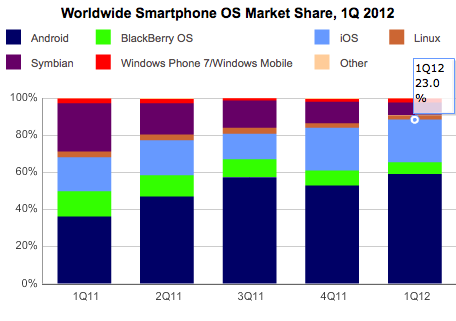
\includegraphics[scale=0.8]{imgs/market-share-2012q1.png} 
	\caption{Participación de iOS en el mercado de sistemas operativos para Smartphones. Fuente \cite{sota:market-smartphones}}
	\label{market-share-2012q1}
\end{figure}



%¿Cuáles son las áreas de investigación y desarrollo de WSN?
%buscar como continuar después de una itemezación con dos puntos y separados por comas.

%Presentar el tema del ruteo y recolección de datos

%IR DE LO GENERAL A LO PARTICULAR!
%El capítulo de introducción debe comenzar explicando que son las 	WSNs.
	%\section{Redes de sensores inalámbricos}
	
	%\section{Aplicaciones}
%En el mundo

%En Chile

	%\section{Protocolo de ruteo para un sistema de recolección de datos}
	%\section{Visión general de los requerimientos}
%Hablar de la aplicación objetivo y cuáles son sus requerimientos 

%Títulos alternativos
% El objetivo de este trabajo es implementar un protocolo de ruteo multihop como parte de un sistema de recolección de datos que está construido sobre una red de sensores inalámbricos. Este sistema está orientado principalmente al monitoreo de variables físicas principalmente relacionadas con la agricultura, como la humedad y la temperatura de los suelos, en zonas de difícil acceso y que no cuentan con redes de distribución eléctrica.

%En el marco de este trabajo, los objetivos generales son los siguientes:
%\begin{enumerate}
%  \item Informar sobre los protocolos de ruteo de mensajes para redes de sensores inalámbricos.
%  \item Desarrollar una red de sensores inalámbricos, utilizando la plataforma de hardware TmoteSky.
%  \item Desarrollar una aplicación para la recolección de datos de la red.
%  \item Evaluar el consumo energético de la red implementada.
%\end{enumerate}

% El primer objetivo se desarrolla en profundidad en el capítulo 2. El segundo objetivo se desarrolla en los capítulos 3, 4 y 5, donde se plantea un diseño de protocolo y posteriormente como se implementa éste. El tercer objetivo se desarrolla en los capítulos 3 y 5 como parte de las verificaciones del sistema. Finalmente, en el capítulo 5 se evalúa el consumo energético el protocolo.\\
 
	%\section{Estado del Arte}


%\subsection{Protocolo de ruteo}
%\begin{figure}[H]
 %\centering
 %\includegraphics[scale=0.8]{imgs/PilaModeloOSI.eps}
 %\caption{Pila de red establecida por el Modelo OSI}
%\end{figure}

	% \subsection{Algoritmos de ruteo propuestos en la literatura}

%En esta sección debería dar una breve reseña  de cada protocolo, con sus referencias.
	%\subsection{Protocolos implementados}

	%\subsection{Hardware de desarrollo}
%De lo general a lo particular
% Qué tipo de hardware existe?

%Debo incluir info sobre los motes que soportan tinyos
	% \subsubsection{Plataformas TinyOS}
	%\subsubsection{Plataformas Zigbee}
	
%Debo incluir info sobre los motes que soportan Zigbee, simpliciti.
	% \subsubsection{Otras plataformas}
	%\subsection{Software para redes de sensores inalámbricos}

%TinyOS, ZStack, SimpliciTI, etc
%Breve descripción de tinyOS e indicación para revisar el anexo XX.
	%\subsubsection{TinyOS}
	%\subsubsection{Contiki}

%Breve descripción de ZStack, basarse en pagina de ti del zstack
	%\subsubsection{Z-Stack}

%Breve descripción de SimpliciTI, basarse en pagina de ti de simpliciti
	% \subsubsection{SimpliciTI}

%Breve descripción de la de los sunspots, basarse en documentacion
	%\subsubsection{Java y SunSpot}

%Breve descripción de alguna otra de otro fabricante..freescale o atmel.

